\documentclass[a4paper,14pt]{article}

\usepackage[14pt]{extsizes}
\usepackage{cmap}					% поиск в PDF
\usepackage{mathtext} 				% русские буквы в формулах
\usepackage[T2A]{fontenc}			% кодировка
\usepackage[utf8]{inputenc}			% кодировка исходного текста
\usepackage[english,russian]{babel}	% локализация и переносы
\usepackage{graphicx}
\usepackage{geometry}
\usepackage{amsmath}
\usepackage{amssymb}
\usepackage[table]{xcolor}
\setlength\extrarowheight{2pt}


\geometry{verbose, a4paper, tmargin=2cm, bmargin=2cm, lmargin=2cm, rmargin=2cm}
\author{Vysotsky Maxim}
\title{Отчёт}
\date{2025}

\begin{document}
	\begin{titlepage}
		\begin{center}
			{Министерство науки и высшего образования Российской Федерации
				НОВОСИБИРСКИЙ НАЦИОНАЛЬНЫЙ ИССЛЕДОВАТЕЛЬСКИЙ
				ГОСУДАРСТВЕННЫЙ УНИВЕРСИТЕТ (НГУ)}
		\end{center}
		\begin{center}
			{Физический факультет}
		\end{center}
		\begin{center}
			{Кафедра общей физики}
		\end{center}
		
		
		\vspace{7cm}
		{
			\begin{center}
				{\bf Лабораторная работа №3.3}\\
			Исследование ударных волн в газах
			\end{center}
		}
		\vspace{2cm}
		\begin{flushright}
			{Руководитель:\\ Ассистент\\
				Художитков В. Э.\\
                Старший преподаватель \\
                Кравцова А. Ю.\\
				Работу выполнил:\\
				Высоцкий М. Ю.\\
				\vspace{0.2cm}
				гр. 24301}
		\end{flushright}
		\vspace{3cm}
		\begin{center}
			Новосибирск, 2025
		\end{center}
	\end{titlepage}

\section{Теоретическое введение}
\hspace{\parindent}\textbf{Цель работы:} знакомство с методами получения и регистра-
ции ударных волн и ударноволновой методикой тарировки пьезодатчиков.

\textbf{Оборудование:} лабораторная ударная труба, пьезодатчики,
усилители, цифровой осциллограф.

Ниже приведена схема установки.

\begin{figure}[h]
    \centering
    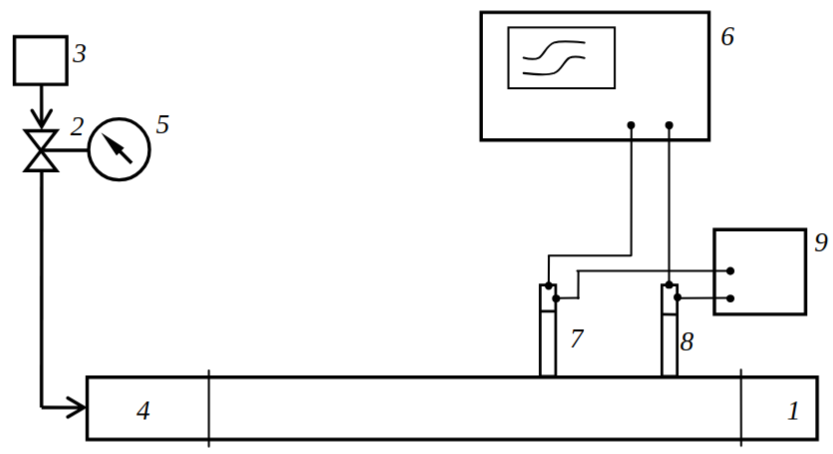
\includegraphics[scale=0.5]{scheme.png}
    \caption{Схема установки. 1 - секция низкого давления, 2 - редуктор давления, 3 - компрессор, 4 - секция высокого давления, 5 - манометр, 6 - осциллограф, 7, 8 - датчики давления, 9 - источник питания датчиков.}
\end{figure}

Скорость звука в идеальном газе:
$$
c = \sqrt{\gamma\frac{RT}{\mu}}
$$

Связь давления в фронте $p_2$ и начального давления $p_1$ перед фронтом:
\begin{equation}
    \frac{p_2}{p_1} = \frac{2\gamma M^2 - (\gamma-1)}{(\gamma+1)}
\end{equation}

Число Маха:
\begin{equation}
    M =\frac{D}{c}
\end{equation}

\clearpage

Связь давления во фронте ударной волны $p_2$ и давлением в камере высокого давления:
\begin{equation}
    \frac{p_2}{p_4} = \left[ 1-\frac{\gamma-1}{\gamma+1} \left( \frac{M^2-1}{M} \right) \frac{c_1}{c_4} \right]^\frac{2\gamma}{\gamma-1}
\end{equation}

Зависимость p4/p1:
\begin{equation}
    \frac{p_4}{p_1} = \frac{\left(\frac{2\gamma M^2}{\gamma + 1}\right)-\left(\frac{\gamma-1}{\gamma+1}\right)}{\left[ 1-\frac{\gamma-1}{\gamma+1} \left( \frac{M^2-1}{M} \right) \frac{c_1}{c_4} \right]^\frac{2\gamma}{\gamma-1}}
\end{equation}

\subsection{Ход работы}

Далее приведены данные эксперимента. $p_4$ - давление, подаваемое в камеру высокого давления, $p_1$ - давление в камере низкого давления (1 атм.), $p_2$ - давление фронта ударной волны, $p_T$ - давление вблизи торца ударной трубы после отражения от
него падающей ударной волны. В данной работе мы принимаем газ за идеальный а также принебрегаем изменением температуры (она равна во всех участках волны). В общем случае, процесс политропный, а в нашем случае - адаиабатический. Для воздуха показатель адиабаты $\gamma$ = 1,4.

\begin{table}[h]
    \centering
    
    \begin{tabular}{|c|c|c|c|}
        \hline 
        $p$, кгс & $\Delta t$, мкс & $v$, м/с & $M$ \\ \hline
        18 & 628 & 398,09 & 1,17 \\  \hline
        35 & 580 & 431,03 & 1,27 \\  \hline
        51 & 552 & 452,90 & 1,33 \\  \hline
        66 & 524 & 477,10 & 1,40 \\  \hline
        83 & 508 & 492,13 & 1,45 \\  \hline
    \end{tabular}
    \caption{Определение числа Маха для 1-5 атмосфер $p_4$}
\end{table}

\clearpage

\begin{table}[h]
    \centering
    
    \begin{tabular}{|c|c|c|c|c|} \hline
        $p_4/p_1$ & $p_2/p_1$ & $p_2/p_4$ & $\Delta p_2$, атм & $\Delta p_t$, атм\\ \hline
        2,09 & 1,43 & 1,37 & 0,43 & 1,02 \\ \hline
        3,06 & 1,71 & 1,68 & 0,71 & 1,81 \\ \hline
        3,88 & 1,90 & 1,96 & 0,90 & 2,43 \\ \hline
        5,01 & 2,13 & 2,12 & 1,13 & 3,20 \\ \hline
        5,85 & 2,28 & 2,34 & 1,28 & 3,74 \\ \hline
    \end{tabular}
    \caption{Расчет давлений $p_2$, $p_4$, $p_t$}
\end{table}

При первом проведении опыта не были сняты показания напряжений с пьезодатчиков. При повторном проведении опыта были сняты следующие показания:

\begin{table}[h]
    \centering
    \begin{tabular}{|c|c|} \hline
        A1, мВ & А2, мВ \\ \hline
        220	& 200 \\ \hline
        600	& 500 \\ \hline
        700	& 620 \\ \hline
        980	& 760 \\ \hline
        1120 & 880 \\ \hline
    \end{tabular}
\end{table}

Имея эти данные, получаем чувствительность первого и второго датчика:
$$
A1 = \frac{1120-220}{2,28-1,43} \approx 1065 \frac{мВ}{атм}
$$

$$
A1 = \frac{880-200}{2,28-1,43} \approx 805 \frac{мВ}{атм}
$$



Далее приведены зависимости $p_4/p_1(M)$, $p_2/p_1(M)$. 

\begin{figure}[h]
    \centering
    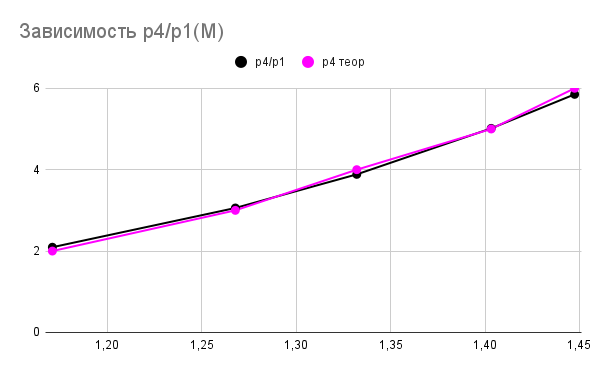
\includegraphics[scale=0.7]{p4p1.png}
    \caption{Зависимость $p4/p1(M)$}
    \label{result}
\end{figure}

\begin{figure}[h]
    \centering
    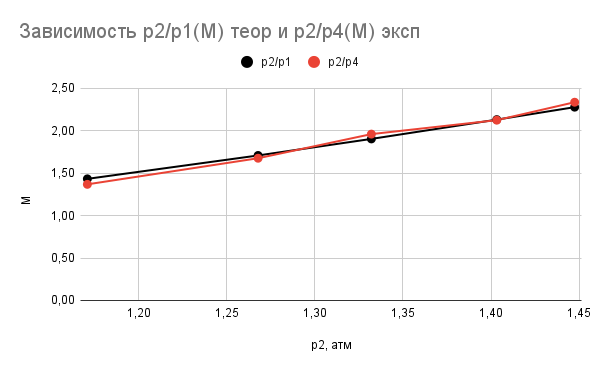
\includegraphics[scale=0.7]{p2p1.png}
    \caption{Зависимость $p2/p1(M)$}
\end{figure}

\clearpage

Также ниже представлены тарировочные кривые для $p_2 - p1$ и $p_Т - p_2$.
\begin{figure}[h!]
    \centering
    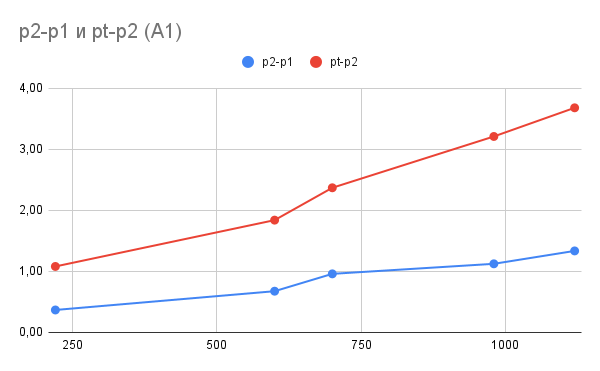
\includegraphics[scale=0.7]{A1.png}
    \caption{Тарировочная кривая для A1}
\end{figure}

\begin{figure}[h!]
    \centering
    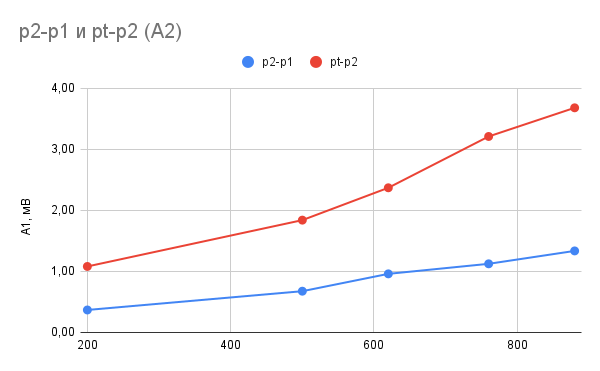
\includegraphics[scale=0.7]{A2.png}
    \caption{Тарировочная кривая для A2}
\end{figure}

\section{Вывод}

Главным выводом в данной работе является то, что зависимость давления $p_4$ от числа Маха растет экспоненциально, что показано на графике (\ref{result}).

\end{document}
